\documentclass{article}
\usepackage{tikz}
\usepackage[margin=0.5in]{geometry}

\usepackage{amsmath}
\begin{document}

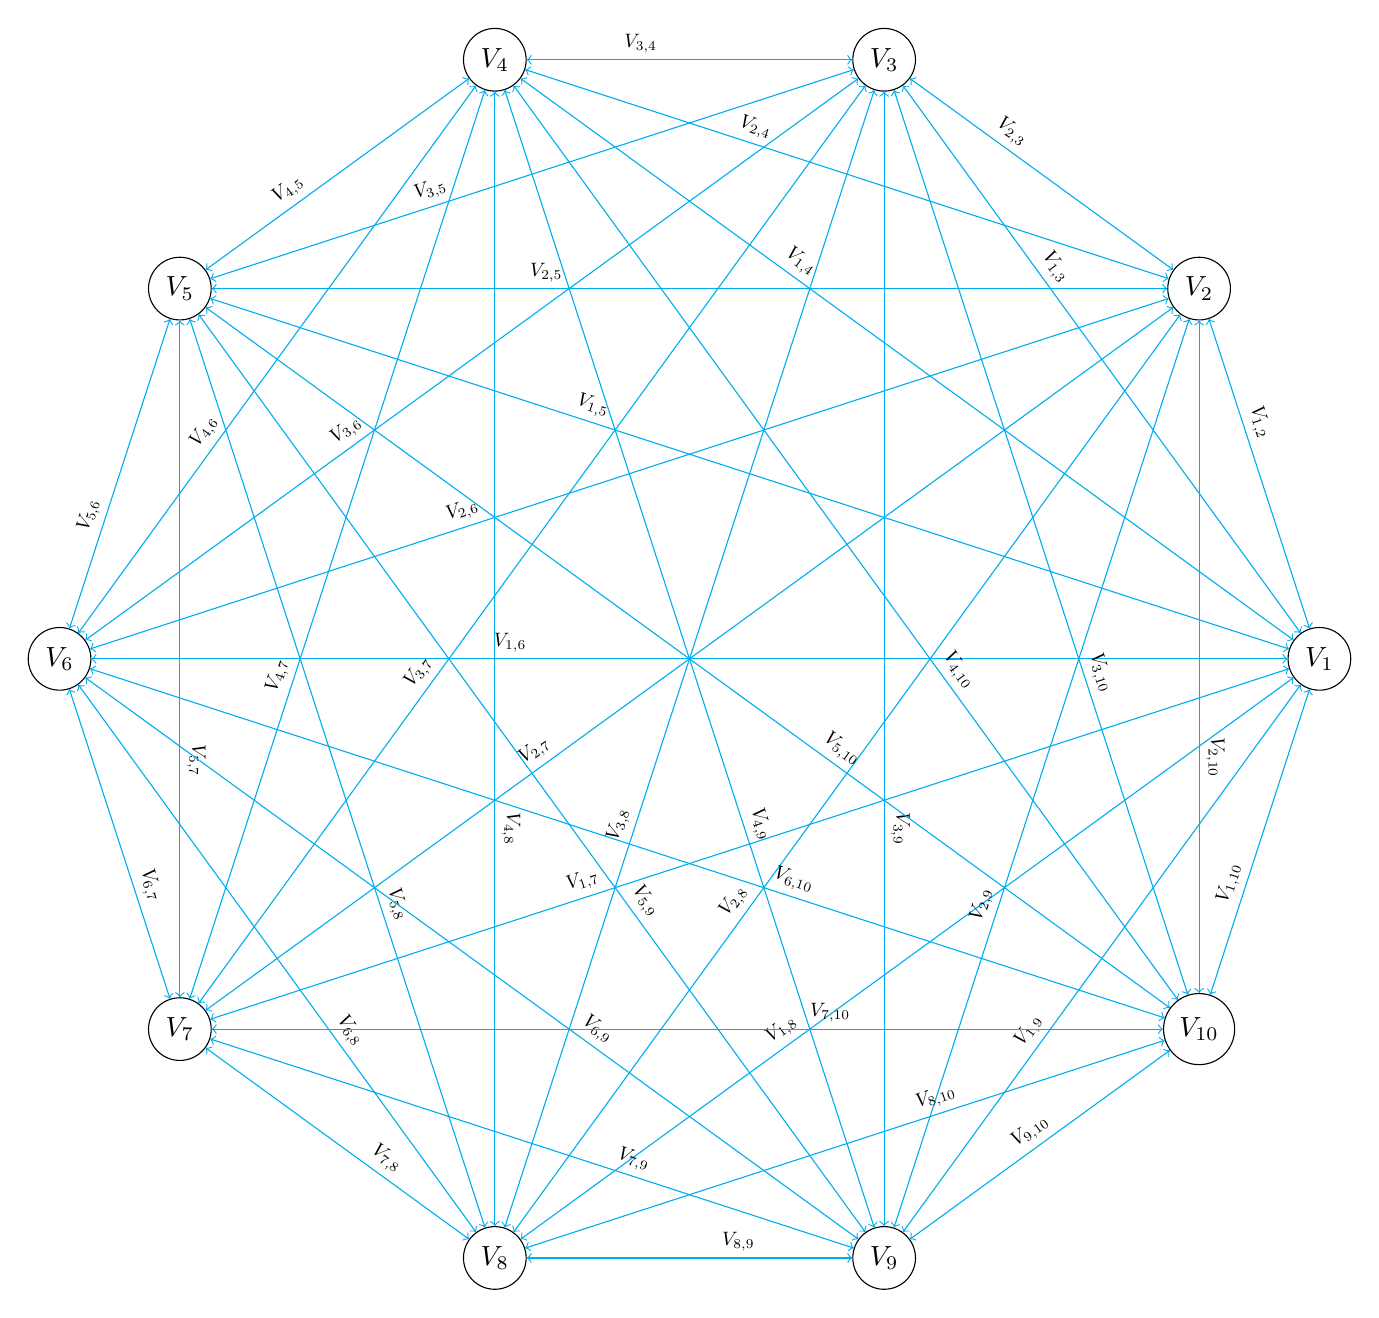
\begin{tikzpicture}[scale = 1]
	\centering

	\pgfmathsetmacro {\n}{10};
	\pgfmathsetmacro{\d}{360/\n};
	\pgfmathsetmacro{\l}{360-\d};
    \foreach \x in {0,\d,...,\l} {
		\pgfmathsetmacro{\a}{int(round((\x + \d)/\d))};
		\node[shape=circle,draw=black] (\a) at (\x:8cm) {$V_{\a}$};
		}
		
		\pgfmathsetmacro{\g}{int(round((\l - \d)))};
		\pgfmathsetmacro{\f}{int(round((\l - 2*\d)))};
		\foreach \x in {0,\d,...,\f} {
		\pgfmathsetmacro{\a}{int(round((\x + \d)/\d))};
		\pgfmathsetmacro{\h}{int(round((\x + \d)))};
		\pgfmathsetmacro{\i}{int(round((\x + 2*\d)))};
		
		 	\foreach \y in {\h,\i,...,\l} {
				\pgfmathsetmacro{\b}{int(round((\y + \d)/\d))};
				\begin{scope}[every node/.style={scale=.7}]
				\path[-latex]
				(\a) edge[<->,cyan] node[above,sloped,color = black,pos = 0.65] {$V_{\a,\b}$} (\b);
				\end{scope}
				
						}
										}
		\pgfmathsetmacro{\g}{int(round((\l - \d)/\d + 2))};
		\pgfmathsetmacro{\f}{int(round((\l - 2*\d)/\d + 2))};								
					\begin{scope}[every node/.style={scale=.7}]
					\path[-latex]
				(\f) edge[<->,cyan] node[above,sloped,color = black] {$V_{\f,\g}$} (\g);			
					\end{scope}
\end{tikzpicture}
\end{document}
